\chapter{System Design}


\section{Design Challenges}
\label{sec:design_challenges}
In the early stages of project, three main challenges were identified: Gut sound monitoring, energy efficiency and wireless connectivity. The problem with these three challenges is that they cannot be faced independently but have to be seen in a common context, as they are tightly coupled with each other. A design decision that is made in one area on behalf of one of the challenges will affect both other fields. 

\begin{figure}
\centering
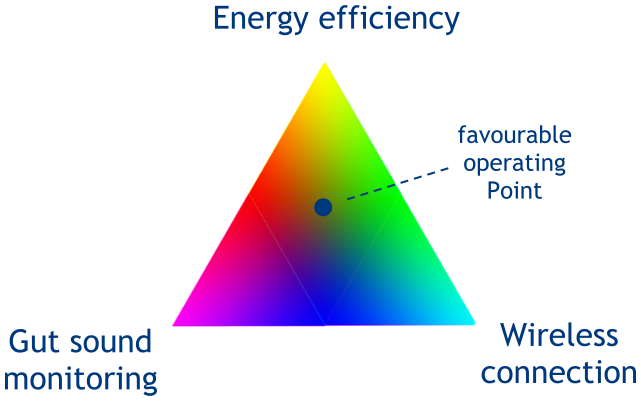
\includegraphics[width=0.8\textwidth]{Images/design_challenges}
\caption{System design challenges}
\label{fig:design_challenges}
\end{figure}

Figure \ref{fig:design_challenges} shows one  way to visualize this three-way tradeoff - it is impossible to design a system with a very high energy efficiency that performs high quality gut sound monitoring and transmits data wirelessly at the same time, because the design space doesn't contain an operating point for this configuration. 

An example for this is our goal to be very energy efficient, because battery life is highly important for mobile devices. Aiming for high energy efficiency puts a constraint on the available choices for a wireless connection, because many wireless protocols are rather energy hungry. At the same time it limits the amount of processing that can be done on the monitoring device, because a busy processor consumes a lot of energy and the aim is to keep the processor sleeping for as long as possible. The cases where sending a larger block of data over wireless is actually more energy-efficient than processing the data on the monitoring device and sending less data over wireless are good illustrations of this tradeoff. 

In order to come up with a design solutions for the main challenges a design space analysis was conducted, where the team attempted to find an operating point close to the center of the design space triangle. The tradeoffs that were taken into consideration will be explained in more detail in the following paragraphs.  

Energy efficiency and the inconveniences caused by the lack of it were mentioned before. One major design goal is a long battery runtime which can only be achieved if every component of the monitoring device is optimized for low power usage. This limits the available choices for the wireless communication protocol and also puts a constraint on the amount of data processing that can be done on the monitoring device.
 
Wireless communication between the monitoring device and the base station is another important issue. A wireless protocol solution which satisfies the bandwidth requirements (audio transmission) while consuming only very little energy is desired. 

Gut sound monitoring is the last of the main design challenges. To be able to do any kind of examination based on the audio data, the length of the recording has to be in the minute range. This requires a wireless protocol with a bandwidth that allows to transmit the data in a reasonable amount of time and limits the processing that can be done during recording because the processor should not be involved in the optimal case.

\TODO{Rewrite/Extend next paragraph}

After discussions and research, a good compromise was found which offers a reasonable degree of fulfillment for each challenge.


\section{Proposed System}
The system that we propose to tackle the design challenges is a distributed system, consisting of wireless monitoring devices optimized for low energy consumption and stationary base station that collects data from monitoring devices and presents it to the user over a web interface. 

This design stands in contrast to the first proposal for the system design in which there is no distinction between monitoring station and base station and the user interacts directly with the system over a wireless protocol commonly available in handheld devices and laptops (Bluetooth) or connects to the device via USB. We realized early that this design was suboptimal, as it is neither scalable nor suited for running on battery power over an extended period of time as Bluetooth is an energy hog and the data processing cannot be offloaded but has to be performed on the device itself.

Separating the roles in the system into distinct devices gives the possibility to design nodes that are optimized for their role in the overall system, which is especially important in this case, as  one of the key focus areas of this project is to build a battery powered device with a long battery runtime. This can only be achieved if the goal is kept in mind during all stages of the design - from the selection of the used components to the design of the system software.


\subsection{Distributed system}
\begin{figure}[htb]
\centering

\includegraphics[width=\textwidth]{Images/dummy}
\caption{Block Diagram: Distributed system}
\label{fig:block_system}
\end{figure}

Figure \ref{fig:block_system} shows  block diagram of the proposed system consisting of multiple monitoring devices and a base station. 
The base station is a stationary device connected to a constant energy source. It provides the network for wireless communication between monitoring devices and the base station. Measurement data from monitoring devices is received over this network, and stored in an internal database. It serves as a common access point for users to retrieve the collected data from multiple monitoring devices and provides easy access from a wide range of devices by presenting the collected data via a web interface.

The monitoring device is a portable battery powered device that can be attached to horses with a strap, and features a range of sensors, a digital stethoscope and means for temporal data storage. The collected data is transferred periodically to the base station, or preserved for later transmission in the local data storage, if the base station is out of reach.

Data access is provided to the user by the base station over a web-interface that displays the collected data and allows the user to download a database for detailed analysis. The audio recordings are stored on an flash memory card in the monitoring devices, and only transferred to the base station of the user requests a data transfer.

\subsection{Wireless connection between nodes}
\label{sec:wireless_connection}
When the decision was made that a distributed system will be developed this also meant that the collected data has to be transmitted wirelessly to the base station, which is as not straightforward as it sounds, given the constraints imposed by the other main challenges that were discussed in section \ref{sec:design_challenges}.

A wireless protocol that had very low energy consumption while offering enough bandwidth to transfer audio signals and supported a range of around 100m was required to adhere the project goals.

In the end the choice fell on the ZigBee protocol, which came closest to fulfilling our feature wish list. The main factors that influenced our decision were
\begin{itemize}
\item Range: up to 100m
\item Power consumption: very low, as it is specifically designed for low-power applications
\item Bandwidth: up to 250kB/s
\item Complexity: easy to setup and use
\end{itemize}

The system is designed in such a way, that monitoring devices have to establish a connection with the base station if they want to transmit data. For energy saving reason, the monitoring devices put their ZigBee modules to sleep when they are not actively transmitting data. This means that the base station cannot send data (commands/requests) to the monitoring devices at arbitrary points of times. It has to wait until a monitoring device connects to the base station before it can dispatch messages. 

